\documentclass[letterpaper]{article}
\usepackage{aaai17}
\usepackage{times}
\usepackage{helvet}
\usepackage{courier}
\usepackage{url}
\usepackage{graphicx}
\usepackage{amsmath}
\usepackage{algorithm2e}
\graphicspath{{images/}}
\frenchspacing  %Required
\setlength{\pdfpagewidth}{8.5in}
\setlength{\pdfpageheight}{11in}

\pdfinfo{
	/Title (Improving Robustness in Social Fabric-based Cultural Algorithms with Two New Approaches in Population and Belief Spaces)
	/Author (Bahram Zaeri and Ziad Kobti)}
\setcounter{secnumdepth}{0}  


\begin{document}
\title{Improving Robustness in Social Fabric-based Cultural Algorithms with Two New Approaches in Population and Belief Spaces}
\author{Bahram Zaeri \and Ziad Kobti\\
School of Computer Science, University of Windsor\\
Emails: \{zaeri, kobti\}@uwindsor.ca}

\maketitle
\begin{abstract}
Robustness is one of the most significant issues when designing evolutionary algorithms. These algorithms should be able to resist against fluctuating responses through the search process. In this paper, we aim at improving Social Fabric-based Cultural Algorithms in both belief space and population components regarding robustness. At first, we propose an irregular neighborhood restructuring mechanism to make the communications between individuals more flexible and let them decide on their exploration or exploitation tendencies through the search process. This method improves the robustness of the search behavior in a self-organized manner. Then, inspired from Inferential Statistics, we utilize the concept of Confidence Interval to propose a new normative knowledge source which is more stable against sudden changes in the values of incoming solutions. The performance of both approaches is measured based on the IEEE-CEC2015 testbed. Compared to the best-known results of other algorithms, our proposed methods showed higher performance on a diverse landscape of numerical optimization problems.
\end{abstract}

\section{Introduction}
Cultural Algorithms (CA) were introduced by Reynolds as a type of population-based problem-solving approaches. CA combines biological evolution with socio-cognitive concepts to yield an optimization approach based on a dual inheritance theory \cite{reynolds1994introduction} \cite{kennedy2001swarm}. A large number of CA variants have been proposed in the literature. They address a vast range of problems such as real-valued function optimization, discrete problems, dynamic environments and multi-objective optimization \cite{RaeesiN.2014}, \cite{reynolds2008computing}, \cite{che2010robust}. \newline In CAs, evolution occurs at two levels: Macro-evolutionary level or belief space and micro-evolutionary level or population space. At the population level, any population-based algorithm such as Genetic Algorithm (GA), Evolutionary Programming (EP), Paricle Swarm Optimization (PSO) could be deployed. The belief space extracts a generalized knowledge from individuals experience to bias the search direction at the population level. This process is accomplished through deploying any of five types of knowledge sources (KSs) in the belief space. Each individual in the population space is controlled by a knowledge source. \newline 
Social Fabric is the notion of an infrastructure in which knowledge sources in the belief space can access the social networks in which individuals interact \cite{reynolds2008social}. Knowledge sources are allowed to propagate their influence on the individuals through a hierarchy of layered networks. Each individual might exist in several networks. As a result, some individuals can play the role of mediator between different networks. \newline
Individuals could be connected in a variety of different topologies. These topologies determine the extent to which the influence of a knowledge source could be propagated through the network \cite{ali2011boosting}. Dense topologies help the individuals to follow (exploit) elite members efficiently while sparse topologies are suitable for exploratory communities \cite{mendes2004population}. To make the propagation of knowledge between individuals more efficient, some neighborhood restructuring schemes are considered by the current extension of CA. Current topologies of networks may transform between different structures to increase/decrease their connectivity rate in the case of stagnation \cite{ali2016leveraged}. \newline
PSO could be considered as another population-based algorithm which relies on social structures. PSO simulates the social behavior observed in natural systems such as birds flocking, herds and schools \cite{kennedy2011particle}. PSO finds the best solution by adjusting the moving vector of each individual (particle) according to its best history and its neighborhood best positions of particles in the entire swarm at each iteration. The neighborhood is determined by the topology of the swarm. For example, dense topologies lead to more interactions and faster convergence. Here, we utilize PSO algorithm at the population level of the CA. As both of the social fabric and PSO approaches use the same social structure for agents communications, we hypothesize that their combination would enhance the social behavior which can lead to improved overall search performance. \newline
In this paper, we aim at improving the robustness of CAs at the both levels of belief space and population space. In the belief space, the standard implementation of Normative ranges will be replaced with the confidence interval concept. This approach makes the normative knowledge source robust against sudden changes in input data. In the population space, the standard tactical neighborhood restructuring is enhanced to a strategy called irregular neighborhood restructuring which occurs at the particles level. It aims at improving robustness regarding self-organization aspect.\newline
The rest of the paper is organized as follows: After the introduction, some research works on socially-motivated problem-solving methods are presented. Then, the original idea of social fabric and the multi-layer influence function are discussed. In the next section, we propose two new approaches for robustness improvement in both population and belief components. Finally, the results of performance evaluations are discussed in the section.
\section{Related Works}
Many variants of CAs have been proposed in a vast range of different applications such as single and multi-objective optimization, dynamic problems, social interactions simulation. Here, we are interested in studying Social Fabric phenomena as a modern variant of CAs which aims at function optimization. \newline
\cite{ali2011boosting} replaced the traditional idea of the roulette wheel with the vector voting model to determine the controller knowledge source of individuals in each iteration. They investigated the effect of different homogeneous topologies in a social fabric. They measured this approach on both static and dynamic problems. Their results confirm that there is no best topology which works well for all problems. So, they concluded that heterogeneous topologies should be considered to make the algorithm scalable for complex problems.\newline
\cite{ali2012socio} divided the whole population into multiple sub-populations (tribes) to construct a two-layer network between individuals. As a diversity-preserving measure, they introduced Tactical Neighborhood Restructuring to avoid stagnation in non-linear multi-modal problems. This strategy facilitate the dissemination of knowledge through the network to help the heterogeneous tribes to prevent local optima.\newline
\cite{chen2006tribe} introduced Tribe-PSO algorithm inspired by Hierarchical Fair Competition. They divided the population into some tribes to draw a two-layer model which splits the individuals into two layers: elite and rudimentary. The process of convergence is divided into three phases to ensure a reasonable level of diversity. They evaluated their algorithm on De Jong's test functions. As an application, they used their approach for molecular docking purpose for a test set of 100 protein-ligand complexes.
\newline
\cite{de2009heterogeneous} investigates different types of heterogeneity in PSO algorithm in four categories: neighborhood, update rule, model of influence and parameters. Here, heterogentiy means particles might have follow different rules or have different initial parameters or neighborhood sizes. It helps PSO variants to hold enough diversity and prevent early convergence.\newline
\cite{ali2016leveraged} gives a detailed description of Social Fabric based Cultural Algorithms with neighborhood restructuring. The idea was to investigate the effect of changing neighborhood of sub-populations (tribes) and how it influences the propagation of information through the fabric (network). Communication between tribes happen through the elites of each tribe. In fact, they are mediators between independent tribes.
\begin{figure}[h]
	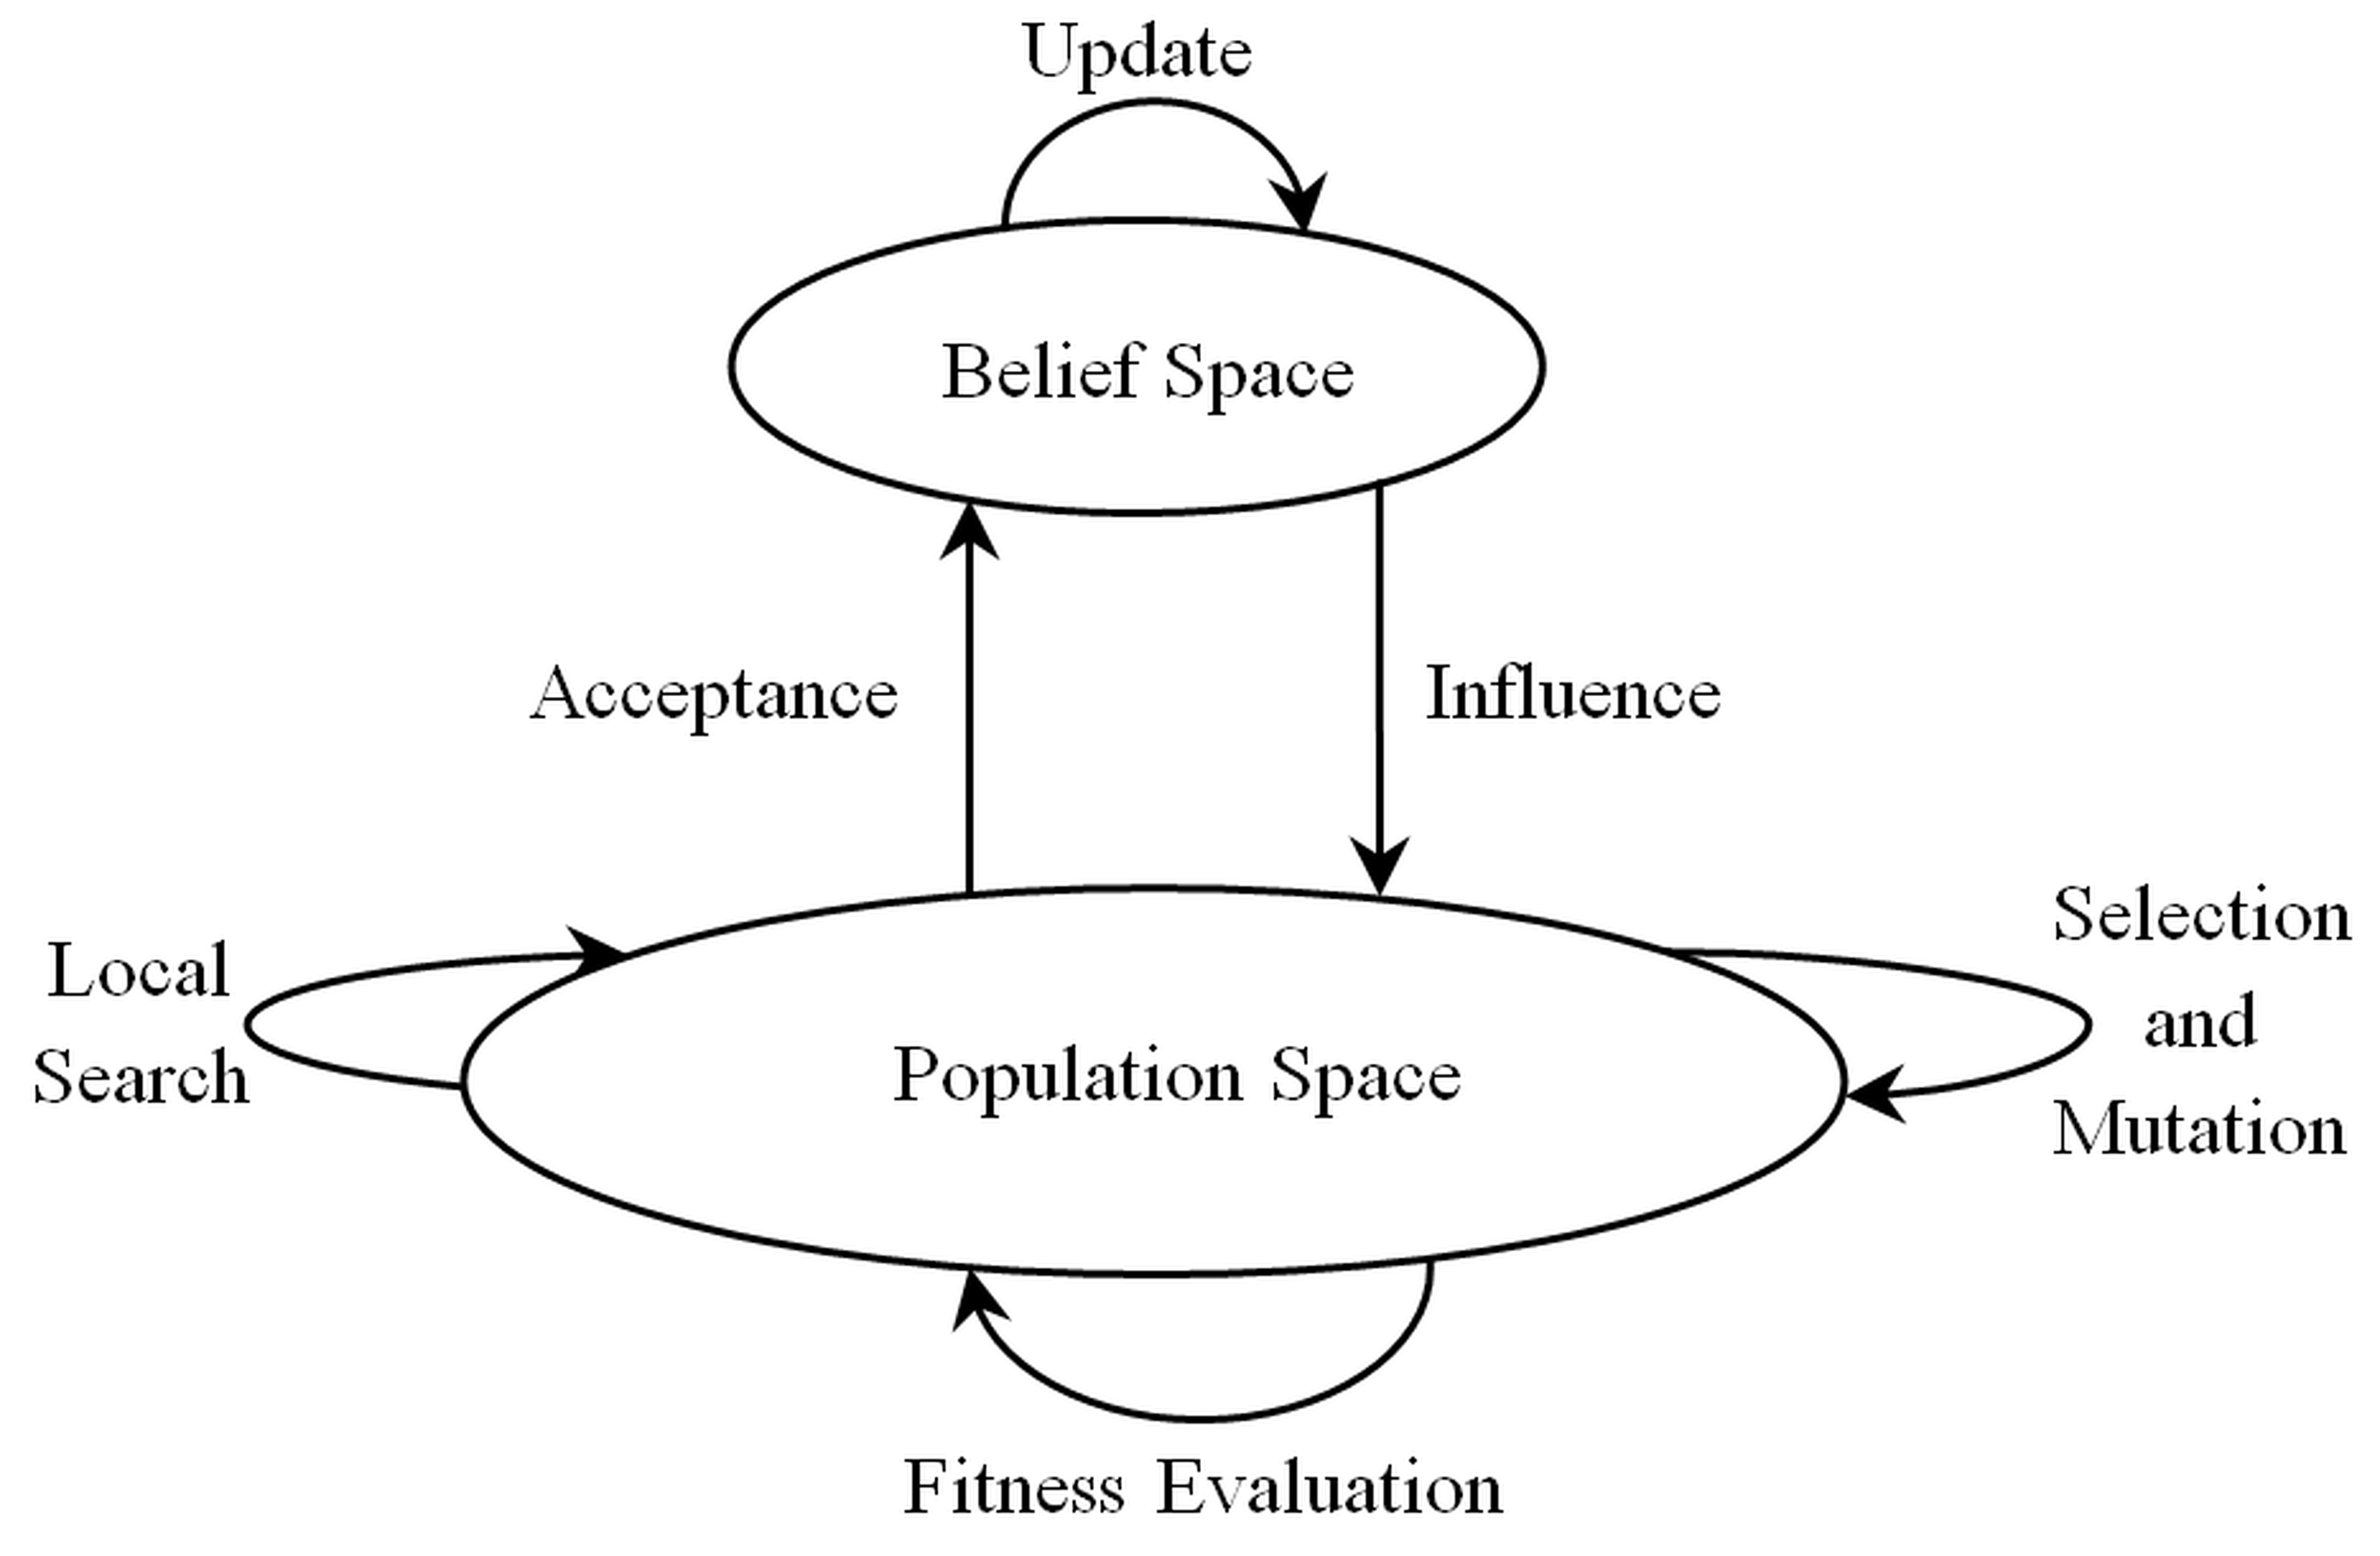
\includegraphics[scale=0.11]{CA}
	\centering
	\caption{Cultural Algorithms \cite{kobti2013heterogeneous}}
	\label{ref:CA}
\end{figure}
\section{Background}
\subsection{Cultural Algorithms}
The figure \ref{ref:CA} shows the basic model of Cultural Algorithms comprised of three components: Population Space, Belief Space and a communication protocol between them. At the population level, any population-based algorithm could be utilized such as GA, EP, PSO. The belief space works as a repository for different types of knowledge acquired from a population. This extracted knowledge is utilized to bias the search process towards the most promising regions of a solution space. While it tries to hold diversity, it prevents the individuals to become divergent. Therefore, it motivates the search behavior in both aspects of exploration and exploitation. Both of the spaces communicate together via communication protocols. It happens through two functions: $accept()$ and $influence()$. The best performing individuals are selected and sent to the belief space by $accept()$ function. Their experience of the chosen individuals will be used to update the belief space. Then, the belief space guides the search behavior through $influence()$ function.
\subsection{Belief Space}
Five types of knowledge sources have been identified in the belief space: the situational KS, the normative KS, the topographic KS, the domain KS and the temporal KS \cite{king2008embedding}. Each knowledge source is responsible for keeping a different type of knowledge about the search process. Domain and Temporal KSs are suitable for dynamic problems. In this paper, static high-dimensional functions are considered. So, we drop Domain and Temporal KSs \cite{ali2016leveraged}.  
\begin{itemize}
	\item Situational Knowledge: It provides a set of exemplary cases to lead the individuals towards the exemplars. So, it is responsible for exploiting the search space. The $X_{i}^{k}(t)$ refers to the $i$th individual of the $k$th tribe at time $t$.
	\begin{equation}
	E(t+1) = \begin{cases} 
				X^{k}_{tELite}(t), & f(X^{k}_{tELite}(t))>f(E(t)) \\ E(t), & \mbox{otherwise} 
			 \end{cases}
	\end{equation}
	
	\item Normative Knowledge: It is a set of promising ranges for parameters values which guide them during the search process to jump into the good range. It is categorized as an exploratory KS. Here, $FR_{j}=[lb_{j}^{t}, ub_{j}^{t}]$ record the range for the $j$th variable and $\lambda=ub_{j}-lb{j}$. $\alpha_{i}$ is a unifrom random variable in $[0, 1]$. $x$ and $x'$ denote the parent and the child solutions respectively.
	\begin{equation}
		x'_{ij}{k}=\begin{cases}
		x_{tElite,j}^{k}(t)+f(X_{i}^{k}(t)) \\ \hspace{35pt} \times \dfrac{\lambda}{\sum_{i=1}^{N}f(X_{i}^{k}(t))}, & x_{ij}{k}(t) \in FR_{j} \\ lb_{j}(t)+\alpha_{i}\cdot (\lambda), & x_{ij}{k}(t) \notin FR_{j}
		\end{cases}
	\end{equation}
	\item Topographic Knowledge: It divides the whole search landscape into cells and keeps tracks of the best individuals in each cell. It aims at digging into promising regions to divide them into smaller subregions. It can be categorized as an exploratory KS because it biases the search process towards promising parts of the search space. $C_{r}$ is the $r$th Cell. $state_{r}(t)\in \{H, L, NE\}$ denotes the diferent states of a topographic cell ($H$ means the cell performs better than average off all cells, while $L$ means it performs worse and $NE$ means, there is no individual in the cell). 
	\begin{equation}
		x'_{ij}{k}=\begin{cases}x_{tElite,j}^k(t)+\dfrac{\alpha_{i}\cdot(u_{r}(t)-l_{r}(t))}{2}, & \\ \hspace{16mm} (x_{ij}{k}\notin C_{r}(t))\wedge(state_{r}(t)\ne L) \\ x_{tElite,j}^k(t)+\dfrac{\alpha_{i}\cdot\sqrt{f(X_{i}^{k}(t))}}{D}, & \\ \hspace{45pt} (x_{ij}{k}(t)\in C_{r}(t))\wedge(state_{r}(t) = H)
		\end{cases}
	\end{equation}
\end{itemize}
\subsection{Social Fabric}
Social Fabric is a dynamic grid of information flow in which the individuals' interactions happen. The fabrics (networks) are created by the connectivity of each agent with other agents in a dynamic structure. The topology of the network controls the rate and type of interactions. Like a multi-population model, there are multiple independent subpopulations (tribes) which are networked together \cite{ali2011boosting}.\newline
\begin{figure}[h]
	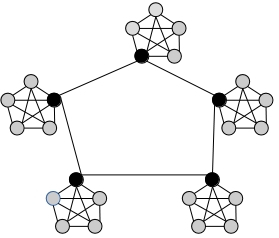
\includegraphics[scale=0.6]{tpso}
	\centering
	\caption{Network structure of Social Fabric and Tribe-PSO}
	\label{ref:tpso}
\end{figure}
In the Social Fabric idea, the influence of the belief space is propagated through the population using a multi-layered network of connections. There are $Z$ tribes comprised of $H$ individuals which form two layers: rudimentary and advanced. The members of each tribe are connected in a regular topology independent from other tribes. At this level, they form the rudimentary layer. From each tribe, the best performing individuals (elites) are connected. These connections create the advanced layer which is responsible for mediating the flow of information between different tribes. Figures \ref{ref:tpso} and \ref{ref:twoLayer} describe the network model.
\subsubsection{Evolution Phases}
The whole evolution process is split into three phases: seclusion, rapport, and cohesive. In the first stage, each tribe evolves as an independent basic CA model with no communication between tribes. In the second step, the advanced layer is formed by connecting elites of each tribe. Then, tribes start to exchange information during their evolution process. Ultimately, in the third step, all the tribes are merged into one CA model. Then the search process continues until meeting some stopping criteria \cite{chen2006tribe} \cite{ali2016leveraged}.
\begin{figure}[h]
	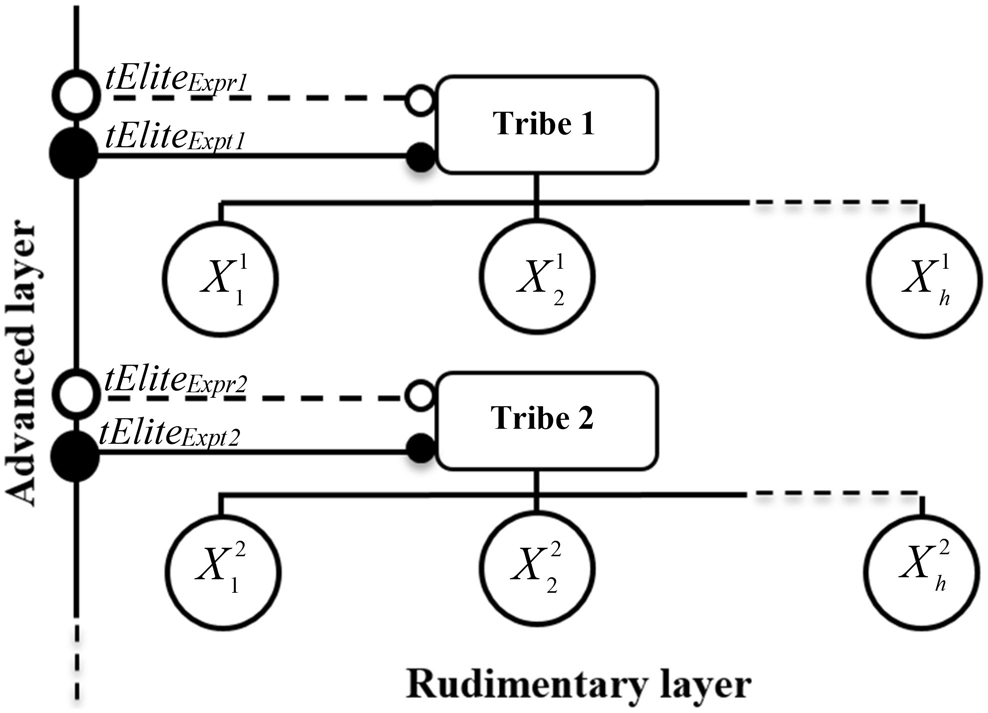
\includegraphics[scale=0.21]{twoLayer}
	\centering
	\caption{Two-layer taxonomy of Tribal model \cite{ali2016leveraged}}
	\label{ref:twoLayer}
\end{figure}
\subsubsection{Strategic Neighborhood Restructuring}
In  Social Fabric literature, Strategic Restructuring is a technique to help individuals to get rid of stagnation where there are copious local optima in the search landscape. Each tribe maintains a particular topology until it gets stagnated in a local optimum for a certain number of iterations. Then, the topology is reinitialized to motivate the individuals for a new search. Here, four types of topologies are utilized: Ring, Mesh, Hybrid-Tree, and Global \cite{ali2012socio} \cite{ali2016leveraged}. \newline
\subsubsection{Social fabric based influence function} In this model, the individuals might decide to change their controller KS using the majority of KSs which they receive from their neighborhood. Here, Majority Voting is used to find the controller KS of an individual \cite{che2010robust}. In the case of a tie, some tie-breaking rules are deployed such as MFU (most frequently used), LFU (least frequently used), Direct (the direct influencing KS), Random (a random choice), Last-used (the KS which controlled the KS in the last iteration) \cite{ali2012socio}. In the equation \ref{eq:4} the sum denotes the counts of KSs in $i$th node neighborhood and $\psi_{i}$ is its contoller KS. $\tau_{i}$ is the net affecting KS for the next iteration \cite{ali2016leveraged} \cite{sterling2004aggregation}. 
\begin{equation}
	\label{eq:4}
	\tau_{i}=\sum_{j \in Nbr(i)}m_{ij} + \psi_{i}
\end{equation}
\section{Particle Swarm Optimization}
In basic PSO, a group of particles (like a flock) is moving around the search space. Each particle is comprised of a position vector and velocity vector \cite{bratton2007defining}. Particles adjust their velocities and positions as follows:
\begin{equation}
	v\textsubscript{id}\textsuperscript{(t+1)}=w\cdot v\textsubscript{id}\textsuperscript{(t)} + c\textsubscript{1}r\textsubscript{1}(p\textsubscript{id}-x\textsubscript{id}\textsuperscript{(t)})+c\textsubscript{2}r\textsubscript{2}(p\textsubscript{gd}-x\textsubscript{id}\textsuperscript{(t)})
\end{equation}
\begin{equation}
	x\textsubscript{id}\textsuperscript{(t+1)}=x\textsubscript{id}\textsuperscript{(t)}+v\textsubscript{id}\textsuperscript{(t+1)}
\end{equation}
Where $v\textsubscript{id}$ and $x\textsubscript{id}$ are the velocity and position of $i$th particle. $c1$ and $c2$ are two positive constants. $r1$ and $r2$ are randomly generated numbers in [0,1] range. $w$ is the inertia weight of which restricts the velocity of a particle. $p\textsubscript{id}$ is the best experience of the particle and $p\textsubscript{gd}$ is the best solution in its neighborhood.
\subsection{Tribe-PSO}
Similar to Social Fabric model, the whole population is divided into some tribes.  The tribes form a two-layer structure of networks, and the whole process consists of three phases. In fact, the idea of Social Fabric originates from Tribe-PSO. But the network structure is utilized to propagate the influence of knowledge sources in the belief space \cite{chen2006tribe}. In this paper, we use the social fabric for both PSO interactions and knowledge propagation of the belief space.
\section{Improving Robustness in Social Fabric}
Inspired by natural systems, many evolutionary algorithms have been proposed to solve various optimization problems. These algorithms are expected to exhibit a consistent problem-solving behavior against different optimization landscapes. Unfortunately, as stated by No Free Lunch (NFL) theorem \cite{wolpert1997no}, there is no algorithm better than others over all cost functions. It means, there is no guarantee for an algorithm to work well for all functions if it shows promising results for a particular category of them. Therefore, robustness has been one of the most desired features which motivates researchers to invent new methods which are less dependent on the kind of a problem than others. Here, robustness means we need to develop search strategies which are capable of adapting themselves across different landscapes which might vary regarding aspects such as multimodality and the number of local optima. 
\newline
In this section, we are going to improve the robustness of CAs in both population space and belief space components. In the population space, a new neighborhood restructuring strategy will be proposed which aims at microscopic inspections for stagnation regarding individuals' local experience. Then, in the belief space, a new model of Normative KS will be proposed, which defines the normative ranges based on Confidence Interval inspired from Inferential Statistics. It stops the normative KS to be affected by sudden fluctuations in the input data.
\subsection{Irregular Neighborhood Restructuring}
As proposed by \cite{ali2016leveraged}, when the agents of a tribe get stuck in a local optimum, then they choose a topology with fewer connections such as ring topology to motivate exploration. When the agents lack information, the topology is changed to a denser topology like Mesh, and ultimately Global. Whenever a tribe does not make progress for $M_{thresh}$ iterations, then the algorithm decides on upgrading/downgrading the current topology to other topologies. Downgrading happens by moving in the direction of gbest$\rightarrow$tree$\rightarrow$mesh$\rightarrow$lbest and Upgrading occurs in the direction of lbest$\rightarrow$mesh$\rightarrow$tree$\rightarrow$gbest. In our proposed approach, the restructuring process occurs at a microscopic level. There is no daemon process for inspecting stagnation. Every agent checks its performance for stagnation. If it gets stuck in a local optimum, it decides to upgrade/downgrade its neighborhood. The proposed strategy is described in the algorithm \ref{ref:RNR}. If the particle is the best in its neighborhood, it starts to decrease the number of connections to motivate exploration. However, if it is not the best, it needs to increase the neighborhood size to facilitate exploitation. Here, the topology is dynamic and irregular and the neighborhood size is different for each agent. So, it could be considered as a heterogeneous variant of CAs \cite{de2009heterogeneous}. The ultimate topology of the fabric is formed through local interactions of the agents. In this way, it improves the robustness of CAs regarding self-organization concept \cite{kennedy2001swarm}. 
\begin{algorithm}{	}
			\caption{Irregular Neighborhood Restructuring}			
				\eIf{$fitness(x\textsubscript{i}) > bestSoFar\textsubscript{i} $}{
					\eIf{$stagnationCounter \ge TiggerThreshold$}{
						\uIf{$x\textsubscript{i} = x\textsubscript{best}$}{
							index = selected randomly from $x\textsubscript{i}$'s neighborhood\newline
							remove $x\textsubscript{index}$ from $x\textsubscript{i}$'s neighborhood
						}
						\Else{
							index = selected from $\{S - x\textsubscript{i}'s neighborhood\}$\newline
							add $x\textsubscript{index}$ to $x\textsubscript{i}$'s neighborhood
						}
						$stagnationCounter = 0$
					}{
					$stagnationCounter = stagnationCounter+1$
				}
			}{
			$stagnationCounter = 0$
		}
		\label{ref:RNR}
\end{algorithm}
\subsection{Confidence based Normative Knowledge Source}
The current version of Normative KS is quite vulnerable to temporary fluctuations in the pattern of input data. The size of Normative ranges is subject to change dramatically with any temporal fluctuations. In this section, we are going to replace the ranges in the standard Normative KS with Confidence Interval from Inferential Statistics. Confidence-based changes are more robust against instantaneous changes in the input pattern. The update process of standard normative ranges is as follows:
\begin{equation}
		lb_{j}(t+1) = \begin{cases} x_{i,j}(t), & x_{i,j}(t)\leq lb_{j}(t)\:or\:f(X_{i})<PL_{j}(t)  \\ lb_{j}, & \mbox{otherwise} \end{cases}
\end{equation}

\begin{equation}
	ub_{j}(t+1) = \begin{cases} x_{i,j}(t), & x_{i,j}(t)\ge ub_{j}(t)\:or\:f(X_{i})<PU_{j}(t)  \\ ub_{j}, & \mbox{otherwise} \end{cases} 
\end{equation}%\newline
The following is the definition of normative ranges based on Confidence Interval concept \cite{proakis1985probability}.
%\begin{equation}
%	(\bar{x}_{j}-q\cdot\dfrac{\sigma_{j}}{\sqrt{n}} , \bar{x}_{j}+q\cdot\dfrac{\sigma_{j}}{\sqrt{n}}) 
%\end{equation}
\begin{equation}
lb_{j}=\bar{x}_{j}-q\cdot\dfrac{\sigma_{j}}{\sqrt{n}}
\end{equation}
\begin{equation}
	ub_{j}=\bar{x}_{j}+q\cdot\dfrac{\sigma_{j}}{\sqrt{n}}
\end{equation}
where 
$\bar{x}$ is mean , $\sigma$ is standard deviation and $q$ is confidence coefficient \newline
\section{Exprimental Results and Analysis}
In this section, the performance of our proposed approaches, on the set of real-world functions specified in the IEEE-CEC2015 expensive optimization test problems \cite{chen2014problem}, is compared with the standard social fabric CA. The algorithms have been implemented in SCALA and have been run with a 2.80 GHz Intel(R) Core(TM) i7-2600S, 8GB RAM, and Linux Ubuntu. The detailed description of the problems is specified in \cite{chen2014problem}. \newline
We set the general parameters the same as described in the standard algorithm \cite{ali2016leveraged}. To implement the irregular neighborhood restructuring strategy, we replaced the EP module in the population component of the standard algorithm with PSO because both of the use social networks to establish the relationships between agents. In this way, both PSO and Social Fabric algorithms utilize the same social structure for communication purpose. For the confidence-based Normative KS, we set the confidence coefficient ($q$) as 1.96.\newline
We have tested our proposed approaches and the standard social fabric algorithm on the IEEE-CEC2015 which is a set of 15 multi-modal and hybrid functions in the form of: 
\begin{equation}
	Y=f(x_{1}, x_{2}, x_{3}, \cdots, x_{D})
\end{equation}
where $D$ is the number of dimensions. Here, we aim at minimizing the results of the functions.\newline
Table \ref{results} shows the evaluation results of the three approaches regarding best, mean, and standard deviation of obtained values. The best obtained results are highlighted in bold. For almost all functions, the proposed approaches work better than the standard version. Based on the reported results, the new restructuring approach generates better mean values in comparison with other approaches. However, regarding the best-generated results, the confidence-based KS outperforms others. The results demonstrate that the proposed ideas enhance the robustness against multi-modality, copious local optima, and etc. For example, the new neighborhood restructuring scheme let the agents develop more connections in promising parts of search space. Here, SFCA stands for the standard social fabric algorithm, ISFCA for the irregular neighborhood restructuring approach and CSFCA for the confidence-based KS approach.
\begin{center}
\begin{table}[htbp]
	\caption{Evaluation Results}
	\begin{center}
		\centering
		\resizebox{\columnwidth}{!}
		{\begin{tabular}{|c|c|c|c|c|}
				\hline
				\multicolumn{1}{|l|}{} & \multicolumn{1}{l|}{} & SFCA & ISFCA & CSFCA \\ \hline
				\multicolumn{ 1}{|c|}{} & Best & 1.058170E+08 & \textbf{5.669974E+02} & 2.070701E+06 \\ \cline{ 2- 5}
				\multicolumn{ 1}{|c|}{T1} & Mean & 2.339E+09 & \textbf{1.346854E+08} & 4.245192E+09 \\ \cline{ 2- 5}
				\multicolumn{ 1}{|c|}{} & Std Dev & 2.398097E+09 & 2.228912E+08 & 6.815361E+09 \\ \hline
				\multicolumn{ 1}{|c|}{} & Best & 2.249944E+04 & 1.939339E+04 & \textbf{1.495766E+04} \\ \cline{ 2- 5}
				\multicolumn{ 1}{|c|}{T2} & Mean & 4.230578E+07 & \textbf{2.772533E+04} & 1.761796E+09 \\ \cline{ 2- 5}
				\multicolumn{ 1}{|c|}{} & Std Dev & 4.249629E+07 & 4.048886E+03 & 3.498278E+09 \\ \hline
				\multicolumn{ 1}{|c|}{} & Best & 3.077165E+02 & \textbf{3.046618E+02} & 3.062800E+02 \\ \cline{ 2- 5}
				\multicolumn{ 1}{|c|}{T3} & Mean & 3.099578E+02 & \textbf{3.052385E+02} & 3.093400E+02 \\ \cline{ 2- 5}
				\multicolumn{ 1}{|c|}{} & Std Dev & 3.298927E+00 & 1.151263E+00 & 2.950910E+00 \\ \hline
				\multicolumn{ 1}{|c|}{} & Best & 1.094153E+03 & 1.301576E+03 & \textbf{6.216136E+02} \\ \cline{ 2- 5}
				\multicolumn{ 1}{|c|}{T4} & Mean & 1.860643E+03 & \textbf{1.340736E+03} & 1.446152E+03 \\ \cline{ 2- 5}
				\multicolumn{ 1}{|c|}{} & Std Dev & 6.769737E+02 & 1.617225E+02 & 8.923725E+02 \\ \hline
				\multicolumn{ 1}{|c|}{} & Best & 5.013705E+02 & 5.013820E+02 & \textbf{5.006284E+02} \\ \cline{ 2- 5}
				\multicolumn{ 1}{|c|}{T5} & Mean & 5.016912E+02 & \textbf{5.016584E+02} & 5.017735E+02 \\ \cline{ 2- 5}
				\multicolumn{ 1}{|c|}{} & Std Dev & 3.171915E-01 & 2.133144E-01 & 1.330542E+00 \\ \hline
				\multicolumn{ 1}{|c|}{} & Best & 6.006698E+02 & \textbf{6.002589E+02} & 6.004211E+02 \\ \cline{ 2- 5}
				\multicolumn{ 1}{|c|}{T6} & Mean & 6.032118E+02 & \textbf{6.004796E+02} & 6.027281E+02 \\ \cline{ 2- 5}
				\multicolumn{ 1}{|c|}{} & Std Dev & 2.292929E+00 & 4.849413E-01 & 2.708244E+00 \\ \hline
				\multicolumn{ 1}{|c|}{} & Best & 7.201798E+02 & \textbf{7.004453E+02} & 7.020742E+02 \\ \cline{ 2- 5}
				\multicolumn{ 1}{|c|}{T7} & Mean & 7.283019E+02 & \textbf{7.016077E+02} & 7.314111E+02 \\ \cline{ 2- 5}
				\multicolumn{ 1}{|c|}{} & Std Dev & 7.886448E+00 & 3.934865E+00 & 3.819154E+01 \\ \hline
				\multicolumn{ 1}{|c|}{} & Best & 9.355662E+03 & 8.067369E+02 & \textbf{8.058631E+02} \\ \cline{ 2- 5}
				\multicolumn{ 1}{|c|}{T8} & Mean & 6.480461E+04 & \textbf{8.112441E+02} & 6.243906E+05 \\ \cline{ 2- 5}
				\multicolumn{ 1}{|c|}{} & Std Dev & 6.170096E+04 & 2.271688E+01 & 1.210907E+06 \\ \hline
				\multicolumn{ 1}{|c|}{} & Best & 9.035692E+02 & 9.036294E+02 & \textbf{9.031234E+02} \\ \cline{ 2- 5}
				\multicolumn{ 1}{|c|}{T9} & Mean & 9.036890E+02 & 9.038236E+02 & \textbf{9.036266E+02} \\ \cline{ 2- 5}
				\multicolumn{ 1}{|c|}{} & Std Dev & 1.100421E-01 & 1.329342E-01 & 4.670059E-01 \\ \hline
				\multicolumn{ 1}{|c|}{} & Best & 1.238238E+04 & 8.895506E+03 & \textbf{2.663896E+03} \\ \cline{ 2- 5}
				\multicolumn{ 1}{|c|}{T10} & Mean & 1.469964E+06 & \textbf{4.313633E+04} & 2.703405E+06 \\ \cline{ 2- 5}
				\multicolumn{ 1}{|c|}{} & Std Dev & 1.495164E+06 & 1.556274E+05 & 4.381762E+06 \\ \hline
				\multicolumn{ 1}{|c|}{} & Best & 1.105861E+03 & \textbf{1.102701E+03} & 1.106682E+03 \\ \cline{ 2- 5}
				\multicolumn{ 1}{|c|}{T11} & Mean & 1.115709E+03 & \textbf{1.104896E+03} & 1.133025E+03 \\ \cline{ 2- 5}
				\multicolumn{ 1}{|c|}{} & Std Dev & 1.497095E+01 & 1.482573E+00 & 4.103627E+01 \\ \hline
				\multicolumn{ 1}{|c|}{} & Best & 1.419774E+03 & \textbf{1.242750E+03} & 1.371989E+03 \\ \cline{ 2- 5}
				\multicolumn{ 1}{|c|}{T12} & Mean & 1.834286E+03 & \textbf{1.251704E+03} & 5.981110E+03 \\ \cline{ 2- 5}
				\multicolumn{ 1}{|c|}{} & Std Dev & 4.350728E+02 & 4.412769E+01 & 8.907798E+03 \\ \hline
				\multicolumn{ 1}{|c|}{} & Best & 1.751179E+03 & \textbf{1.615215E+03} & 1.632836E+03 \\ \cline{ 2- 5}
				\multicolumn{ 1}{|c|}{T13} & Mean & 1.823389E+03 & \textbf{1.621276E+03} & 2.310349E+03 \\ \cline{ 2- 5}
				\multicolumn{ 1}{|c|}{} & Std Dev & 7.164489E+01 & 1.206705E+01 & 8.451440E+02 \\ \hline
				\multicolumn{ 1}{|c|}{} & Best & 1.600443E+03 & 1.601356E+03 & \textbf{1.592262E+03} \\ \cline{ 2- 5}
				\multicolumn{ 1}{|c|}{T14} & Mean & 1.613461E+03 & \textbf{1.602010E+03} & 1.604816E+03 \\ \cline{ 2- 5}
				\multicolumn{ 1}{|c|}{} & Std Dev & 1.593092E+01 & 2.175189E+00 & 1.451758E+01 \\ \hline
				\multicolumn{ 1}{|c|}{} & Best & 1.906632E+03 & \textbf{1.511100E+03} & 1.869629E+03 \\ \cline{ 2- 5}
				\multicolumn{ 1}{|c|}{T15} & Mean & 2.005936E+03 & \textbf{1.571175E+03} & 1.950623E+03 \\ \cline{ 2- 5}
				\multicolumn{ 1}{|c|}{} & Std Dev & 9.865090E+01 & 1.070965E+02 & 8.655941E+01 \\ \hline
			\end{tabular}}
	\end{center}
	\label{results}
\end{table}
\end{center}
\section{Conclusion}
In this paper, two novel strategies were introduced to improve the robustness of CAs in both population and belief spaces. In the first strategy, a new neighborhood restructuring strategy is employed which aims at individuals with irregular and heterogeneous neighborhood structures. There is no centralized coordinator to control the topology of a population because the individuals are responsible for inspecting and modifying their neighborhood in a self-organized manner. Increasing the level of self-organization and autonomy is a key approach to improving robustness in a complex system.  In the second strategy, the standard implementation of normative ranges in the belief space was replaced by the confidence intervals inspired from Inferential Statistics. The new knowledge source shows a more robust search behavior to fluctuations in the input data. Now, the size of normative ranges does not change dramatically with any temporal fluctuations.\newline
The performance of both proposed approaches is assessed through a test-suite of 15 multi-modal and hybrid functions from IEEE-CEC2015. Both methods are compared to the original version of the social fabric based CA \cite{ali2016leveraged}. The results show improvement in almost all of the functions. In some of them, the results are quite promising. Future work might be investigating the improved robustness of proposed approaches to dynamic problems or even real-world problems such as dynamic problems, data classification and social network analysis.
\bibliography{references}
\bibliographystyle{aaai}
\end{document}
